%%% Esqueleto base de la presentacion
%%% No agregar las paginas con un include
%%% Lo que quieran aportar deben ser usuarios del TRAC

\documentclass{beamer}
\usepackage[spanish,activeacute]{babel}
\usepackage[utf8]{inputenc}
\usepackage{listings}
\usepackage{color}
\definecolor{gray2}{rgb}{100,100,100}
\definecolor{red}{rgb}{255,0,0}
\definecolor{green}{rgb}{0,1,0} 
\definecolor{blue}{rgb}{0,0,1} 
\newcommand{\blue}{\textcolor{blue}}
\newcommand{\red}{\textcolor{red}}
\newcommand{\green}{\textcolor{green}}



\usetheme[pageofpages=of,% String used between the current page and the
                         % total page count.
          alternativetitlepage=true,% Use the fancy title page.
          titlepagelogo=img/qt-logo,% Logo for the first page.
          watermark=img/qt-logo-off,% Watermark used in every page.
          watermarkheight=100px,% Height of the watermark.
          watermarkheightmult=4,% The watermark image is 4 times bigger
                                % than watermarkheight.
          ]{Torino}

\usecolortheme{nouvelle}
\vspace{-0.5cm}
\author{\large Cristián D. Maureira Fredes\\\normalsize \textcolor{gray}{saint@archlinux.cl}}
\title{\Huge Introducción a PyQt}
\subtitle{\Large \textit{``¿Quién dijo que crear e implementar interfaces es dificil?''}}
\institute{
	\vspace{0.1cm}
	Comunidad \textbf{KDE} Chile y\\ \textbf{Arch Linux} Chile\\\vspace{0.1cm}
	
\includegraphics[height=0.1\textheight]{img/kde}\hspace{0.1cm}
	
\includegraphics[height=0.1\textheight]{img/arch}
	}

\begin{document}
\begin{frame}[t,plain]
\titlepage
\end{frame}

\begin{frame}
    \frametitle{Introducción}
    \framesubtitle{¿Qué es FMM?}

    \begin{center}
        Es un algoritmo TreeCode que utiliza dos representaciones del campo gravitatorio,
        campos lejanos (multipole) y expansiones locales.
    \end{center}
\end{frame}

\begin{frame}
    \frametitle{Introducción}
    \framesubtitle{¿Por qué es importante?}

    \begin{itemize}
        \item Cálculo muy rápido del potencial (campo).
        \item Más fácil computacionalmente trabajar con el potencial que con la fuerza.
        \begin{itemize}
            \item La fuerza es un vector. $$F_{ij} =G \cdot \frac{m_i \cdot m_j}{||r_{ij}||^{2}} \cdot \frac{r_{ij}}{||r_ij||}$$
            \item El potencial es un escalar. $$\Phi_{i} = \sum_{j=0}^{N} \frac{m_{j}}{r}$$
        \end{itemize}
        \item $F = - \nabla \Phi $
    \end{itemize}
\end{frame}


\begin{frame}
    \frametitle{Introducción}
    \framesubtitle{¿Cuál es la idea?}

    \begin{itemize}
        \item La estrategia es calcular una expresión compacta para el potencial.
        \begin{itemize}
            \item fácil de evaluar con sus derivadas.
        \end{itemize}
        \item Esto se consigue evaluando el potencial como un ``desarrollo multipolar'' (multipole expansion)
        \begin{itemize}
            \item Toma la idea de una expansión de Taylor.
            \item Es exacta cuando el valor de $r^2$ es grande.
                $$r^{2} = x^{2} + y^{2} + z^{2}$$
                  Siendo $r$ la distancia entre dos cuerpos.
        \end{itemize}
    \end{itemize}
\end{frame}

\begin{frame}
    \frametitle{Introducción}
    \framesubtitle{¿En qué se diferencia con un TreeCode?}

    \begin{itemize}
        \item<1-> FMM calcula una expresión para el \blue{potencial} en todos los puntos, no la \blue{fuerza} como lo hace el TC.
        \item<2-> FMM usa \blue{más información} que sólo la masa y el centro de las partículas en una caja.
        \item<2-> Esta expansión compleja es \blue{más precisa}, pero también \red{más cara} si se usan expansiones de mayor orden.
        \item<3-> Decidir si ocupamos la masa y el centro de masa de una caja de lado $n$ en un punto distante,
                  o si tenemos que descomponerla, depende sólo de la \blue{ubicación y tamaño de la caja},
                  \textbf{no} de la \blue{ubicación del centro de masa} de la caja.
    \end{itemize}
\end{frame}

\section{Conceptos}
\frame
{
\frametitle{Conceptos}
\framesubtitle{OO}
\begin{itemize}
	\item Es importante que recordemos la \blue{Orientación a Objetos}.
	\item Es de \red{vital} importancia, para Python y para Qt.
\end{itemize}
}

\frame
{
\frametitle{Conceptos}
\framesubtitle{Jerarquía}
\begin{itemize}
	\item Su estructura es \blue{modular}.
	\begin{itemize}
		\item $>$ 300 clases.
		\item $>$ 6000 métodos.
	\end{itemize}
	\item En los cuales podemos encontrar:
	\begin{itemize}
		\item QtCore
		\item QtGui
		\item QtSvg
		\item QtSQL
		\item ...
	\end{itemize}
\end{itemize}
}

\frame
{
\frametitle{Conceptos}
\framesubtitle{Comportamiento}
\begin{itemize}
	\item Tenemos \blue{Objetos} (elementos)
	\item Tenemos \red{Señales} (por cada elemento) 
\end{itemize}
}

\frame
{
\frametitle{Conceptos}
\framesubtitle{Comportamiento}
\begin{center}
	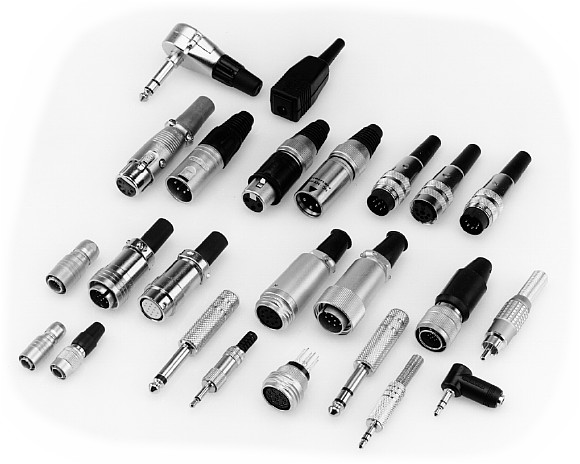
\includegraphics[width=0.5\textwidth]{img/tipos}
\end{center}
}

\frame
{
\frametitle{Conceptos}
\framesubtitle{Comportamiento}
\begin{itemize}
	\item Cada objeto tiene \blue{una o más} señales:
	\begin{itemize}
		\item \emph{connect()}
		\item \emph{valueChanged()}
		\item \emph{textChanged()}
		\item \emph{accepted()}
		\item \emph{triggered()}
		\item ...
	\end{itemize}
\end{itemize}
}

\section{Ejemplos}
\begin{frame}[t,fragile]
\frametitle{Ejemplos}
\framesubtitle{Lineas}
\tiny
\lstset{language=Python}
\lstinputlisting{code/03/lineas-impl.py}
\end{frame}


\begin{frame}[t,fragile]
\frametitle{Ejemplos}
\framesubtitle{Listas}
\tiny
\lstset{language=Python}
\lstinputlisting{code/04/listas-impl.py}
\end{frame}

\begin{frame}[t,fragile]
\frametitle{Ejemplos}
\framesubtitle{Seleccion}
\tiny
\lstset{language=Python}
\lstinputlisting{code/05/seleccion-impl.py}
\end{frame}


\begin{frame}[t,fragile]
\frametitle{Ejemplos}
\framesubtitle{Fuentes}
\tiny
\lstset{language=Python}
\lstinputlisting{code/06/fonts-impl.py}
\end{frame}


\begin{frame}[t,fragile]
\frametitle{Ejemplos}
\framesubtitle{Calendario}
\tiny
\lstset{language=Python}
\lstinputlisting{code/07/calendar-impl.py}
\end{frame}

\begin{frame}[t,fragile]
\frametitle{Ejemplos}
\framesubtitle{Tabs}
\tiny
\lstset{language=Python}
\lstinputlisting{code/08/tabs-impl.py}
\end{frame}

\begin{frame}[t,fragile]
\frametitle{Ejemplos}
\framesubtitle{Formulario}
\tiny
\lstset{language=Python}
\lstinputlisting{code/09/formulario-impl.py}
\end{frame}

\begin{frame}[t,fragile]
\frametitle{Ejemplos}
\framesubtitle{Menu}
\tiny
\lstset{language=Python}
\lstinputlisting{code/10/menu-impl.py}
\end{frame}

\begin{frame}[t,fragile]
\frametitle{Ejemplos}
\framesubtitle{Drag and Drop}
\tiny
\lstset{language=Python}
\lstinputlisting{code/11/dragdrop.py}
\end{frame}

\begin{frame}[t,fragile]
\frametitle{Ejemplos}
\framesubtitle{Multimedia - Audio}
\tiny
\lstset{language=Python}
\lstinputlisting{code/12-multimedia/audio.py}
\end{frame}

\begin{frame}[t,fragile]
\frametitle{Ejemplos}
\framesubtitle{Multimedia - Video}
\tiny
\lstset{language=Python}
\lstinputlisting{code/12-multimedia/video.py}
\end{frame}

\begin{frame}[t,fragile]
\frametitle{Ejemplos}
\framesubtitle{openWall}
\begin{center}
	Veamos el codigo!
\end{center}
\end{frame}

\begin{frame}[t,fragile]
\frametitle{Ejemplos}
\framesubtitle{$\mu$Bot Interface}
\begin{center}
	Veamos el codigo!
\end{center}
\end{frame}

\section{Conclusiones}
\frame
{
\frametitle{Conclusiones}
\begin{itemize}
	\item C++ es un muy buen lenguaje, \blue{pero} Python es más simple.
	\item Qt nos ofrece una \blue{amplia} cantidad de Áreas.
	\item Al unir dos elementos \red{simples}, obtenemos algo genial.
	\item \red{No} es solo un juguete, se pueden hacer cosas serias.
	\item Abundan tutoriales en la red.
	\item Buena documentación.
	\item \red{Fácil} de aprender.
\end{itemize}
}

\frame
{
\vspace{1cm}
\begin{center}
	\Huge{¿Preguntas?}
\end{center}
}


\end{document}








